\documentclass[conference]{IEEEtran}
\IEEEoverridecommandlockouts
% The preceding line is only needed to identify funding in the first footnote. If that is unneeded, please comment it out.
\usepackage{cite}
\usepackage{amsmath,amssymb,amsfonts}
\usepackage{algorithmic}
\usepackage{graphicx}
\usepackage{textcomp}
\usepackage{xcolor}
\usepackage{mathtools}
\usepackage{subfigure}

\def\BibTeX{{\rm B\kern-.05em{\sc i\kern-.025em b}\kern-.08em
    T\kern-.1667em\lower.7ex\hbox{E}\kern-.125emX}}
\begin{document}

\title{Orientation Tracking and Panorama Generation\\

}

\author{\IEEEauthorblockN{1\textsuperscript{st} Pengxi Zeng}
    La Jolla, CA \\
    p2zeng@ucsd.edu}


\maketitle

\begin{abstract}
    This paper presents an approach to solving the Simultaneous Localization and Mapping (SLAM) 
    problem using the Extended Kalman Filter (EKF). The SLAM problem is the task of estimating 
    the position and orientation of a robot as well as the positions of features or landmarks 
    in the environment, while simultaneously building a map of the environment. The EKF is a 
    popular algorithm for estimating the state of nonlinear dynamic systems and is well-suited
    to the SLAM problem due to its ability to handle nonlinear measurement and motion models.
\end{abstract}

\begin{IEEEkeywords}
    SLAM, Extended Kalman Filter
\end{IEEEkeywords}

\section{Introduction}

Simultaneous Localization and Mapping (SLAM) is the problem of estimating the trajectory of a robot and simultaneously building a map of its environment. SLAM is a fundamental problem in robotics and has many applications in autonomous driving, robotics, and augmented reality.

One approach to solving the SLAM problem is to use the Extended Kalman Filter (EKF), which is a popular algorithm for estimating the state of nonlinear dynamic systems. In the context of SLAM, the EKF is used to estimate the pose of the robot (i.e., its position and orientation) as well as the positions of the landmarks in the environment.

The basic idea of EKF-based SLAM is to use sensor measurements (e.g., odometry, laser range-finder data, etc.) to estimate the pose of the robot and update the map of the environment. The EKF operates in a recursive fashion, where it uses the current state estimate and measurements to predict the next state estimate, and then uses this estimate to update the map.

One of the challenges in EKF-based SLAM is that the measurement and motion models are typically nonlinear, which makes it difficult to use the standard Kalman Filter. However, the EKF provides a way to handle nonlinear models by approximating them as linear models around the current state estimate. This allows the EKF to estimate the state of the system even when the models are nonlinear.

Overall, EKF-based SLAM is a powerful approach to solving the problem of robot localization and mapping, and has been successfully used in many real-world applications.


\section{Problem Formulation}
\subsection{General Form}
We usually adopt extened kalman filter to solve SLAM problem. The main difference between common kalman filter and EKF is that
EKF does not require that the model to be linear. In EKF, we assume the prior obeys the normal distribution:
\begin{equation}
    \mathbf{x}_t | \mathbf{z}_{0:t}, \mathbf{u}_{0:t-1} \sim N (\mu_{t|t}, \Sigma_{t|t})
\end{equation}

And the motion model and observation model could be described respectively as follows:
\begin{equation}
    \begin{aligned}
    & \mathbf{x}_{t+1}=f\left(\mathbf{x}_t, \mathbf{u}_t, \mathbf{w}_t\right), \quad \mathbf{w}_t \sim \mathcal{N}(\mathbf{0}, W) \\
    & F_t:=\frac{d f}{d \mathbf{x}}\left(\boldsymbol{\mu}_{t \mid t}, \mathbf{u}_t, \mathbf{0}\right), \quad Q_t:=\frac{d f}{d \mathbf{w}}\left(\boldsymbol{\mu}_{t \mid t}, \mathbf{u}_t, \mathbf{0}\right)
    \end{aligned}
\end{equation}

\begin{equation}
    \begin{aligned}
    & \mathbf{z}_t=h\left(\mathbf{x}_t, \mathbf{v}_t\right), \quad \mathbf{v}_t \sim \mathcal{N}(\mathbf{0}, V) \\
    & H_t:=\frac{d h}{d \mathbf{x}}\left(\boldsymbol{\mu}_{t \mid t-1}, \mathbf{0}\right), \quad R_t:=\frac{d h}{d \mathbf{v}}\left(\boldsymbol{\mu}_{t \mid t-1}, \mathbf{0}\right)
    \end{aligned}
\end{equation}


Thus, from the motion model, we could do the prediction and update step as follows:


\begin{equation}
    \begin{aligned}
    & \mu_{t+1 \mid t}=f\left(\mu_{t \mid t}, \mathbf{u}_t, \mathbf{0}\right) \\
    & \Sigma_{t+1 \mid t}=F_t \Sigma_{t \mid t} F_t^{\top}+Q_t W Q_t^{\top} 
    \end{aligned}
\end{equation}

\begin{equation}
    \begin{aligned}
    & \mu_{t+1 \mid t+1}=\mu_{t+1 \mid t}+K_{t+1 \mid t}\left(z_{t+1}-h\left(\mu_{t+1 \mid t}, 0\right)\right) \\
    & \Sigma_{t+1 \mid t+1}=\left(I-K_{t+1 \mid t} H_{t+1}\right) \Sigma_{t+1 \mid t}
    \end{aligned}
\end{equation}
in which the Kalman gain could be calculated as:
\begin{equation}
    \begin{aligned}
    K_{t+1 \mid t}:=&\Sigma_{t+1 \mid t} H_{t+1}^{\top} \\ &\left(H_{t+1} \Sigma_{t+1 \mid t} H_{t+1}^{\top}+R_{t+1} V R_{t+1}^{\top}\right)^{-1}
    \end{aligned}
\end{equation}



\section{Technical Approach}
\subsection{Pose Prediction}
Consider the localization-only problem, from the motion model, we know the funtion of calculating the pose with twist:
\begin{equation}
T_{k+1} = T_k\exp{\tau_k\hat{\zeta}_k}
\end{equation}

Then the nominal and perturbation could be calculated as:
\begin{equation}
    \begin{aligned}
    \boldsymbol{\mu}_{t+1} & =\boldsymbol{\mu}_t \exp \left(\tau_t \hat{\mathbf{u}}_t\right) \\
    \delta \boldsymbol{\mu}_{t+1} & =\exp \left(-\tau_t \hat{\mathbf{u}}_t\right) \delta \boldsymbol{\mu}_t+\mathbf{w}_t
    \end{aligned}
\end{equation}

And the covariance is:
\begin{equation}
    \begin{aligned}
    &\Sigma_{t+1 \mid t} =\mathbb{E}\left[\delta \boldsymbol{\mu}_{t+1 \mid t} \delta \boldsymbol{\mu}_{t+1 \mid t}^{\top}\right] \\
    &=\exp \left(-\tau \hat{\mathbf{u}}_t\right) \Sigma_{t \mid t} \exp \left(-\tau \hat{\mathbf{u}}_t\right)^{\top}+W
    \end{aligned}
\end{equation}

\subsection{Update}
\subsubsection{Mapping Update}
Since we assume all the features stay static, we don't need to predict the features' poses. The update for the landmarks' 
positions could be formulated as:
\begin{equation}
    \begin{aligned}
    K_{t+1} & =\Sigma_t H_{t+1}^{\top}\left(H_{t+1} \Sigma_t H_{t+1}^{\top}+I \otimes V\right)^{-1}, \\
    \mu_{t+1} & =\mu_t+K_{t+1}\left(\mathbf{z}_{t+1}-\tilde{\mathbf{z}}_{t+1}\right), \\
    \Sigma_{t+1} & =\left(I-K_{t+1} H_{t+1}\right) \Sigma_t,
    \end{aligned}
\end{equation}
where $H_{t+1, i, j} = \mathbb{I}(\Delta_t(j) = i) K_s \frac{d\pi}{d\mathbf{q}}(_{o}T_{w}\underline{\mu}_{t,j})P^{\top}$

\subsubsection{Pose Update}
The two differences between mapping update and pose update are how to calculate $H_{t+1}$ and the rule for mean:
\begin{equation}
    H_{t+1, i}=-K_s \frac{d \pi}{d \mathbf{q}}\left( _oT_i \boldsymbol{\mu}_{t+1 \mid t}^{-1} \underline{\mathbf{m}}_j\right) \prescript{}{o}{T_i}\left(\boldsymbol{\mu}_{t+1 \mid t}^{-1} \underline{\mathbf{m}}_j\right)^{\odot}
\end{equation}
\begin{equation}
    \mu_{t+1} =\mu_t\exp\left((K_{t+1}\left(\mathbf{z}_{t+1}-\tilde{\mathbf{z}}_{t+1}\right)\hat)\right)
\end{equation}

\subsubsection{Simultaneously Update}
The former two updates both assume other contions are correct and static. However, in SLAM, this could lead to a problem that 
the pose and the landmarks are correlated in the process. And the former two updates would lose the covariance information
between the pose and the landmarks.

To update the pose and landmarks' means simultaneously, we need to stack the pose's mean and the landmarks' means. Thus, we 
will have a vector $\mu \in \mathbb{R}^{6 + 3M}$, where 6 represents the robot's position and orientation, and $3M$ represents
the flattened M landmarks' positions. To calculate parameters $H_t$, we just need to separately calculate $H_t^{pose}$ and 
$H_t^{landmarks}$ following the former two parts 
and stack them to form $H_t \in \mathbb{R}^{4N_t\times (6+3M)}$. All other parameters are formed in the 
same way. In the final update step, we could split the residual term $K_{t+1}(z_{t+1} - \tilde{z}_{t+1})$ into two parts 
corresponding to the pose mean and the landmarks mean.

\subsection{Some More Details}
\subsubsection{\textbf{Noise}}
The EKF is sensitive to noise settings. The reasonable magnitude for the motion noise variance should be $[1e^{-1}, 1e^{-5}]$
and for observation noise variance should be $[1e^0, 1e^1]$. And the initial settings for pose $\Sigma_0$ should be very small 
since we are pretty sure of the initial pose. and for landmarks, the magnitude should also be of $[1e^0, 1e^1]$.

\subsubsection{\textbf{Update}}
When updating the landmarks' mean at time $t$, we only choose those entries that corresponds to the landmarks that are observed
at time $t$. It is also the same after $\Sigma_{t+1|t+1}$ is obtained. We will only renew the entries related to 
pose and observed landmarks.

\section{Results}
\subsection{Dead Reckoning}
With only adopting prediction on the pose of the robot and updating the 
positions of the landmarks, the obtained trajectories are as Fig.\ref{fig:dead_reckoning}. I first assume the landmarks 
were completely independent.

\begin{figure}[htbp]
    \centering
    \subfigure[Dataset 03]{
        \begin{minipage}[t]{1\linewidth}
            \centering
            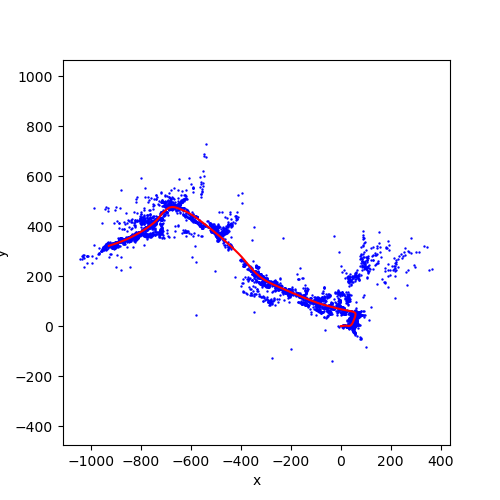
\includegraphics[width=2.5in]{../figs/03_deadreckoning.png}
            % \caption{}
        \end{minipage}%
    }%

    \subfigure[Dataset 10]{
        \begin{minipage}[t]{1\linewidth}
            \centering
            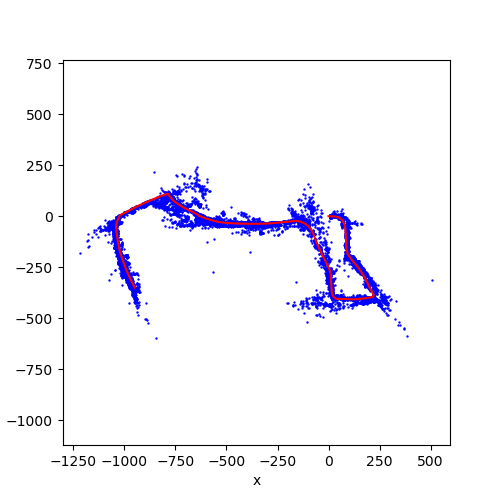
\includegraphics[width=2.5in]{../figs/10_deadreckoning.png}
            % \caption{}
        \end{minipage}
    }%
    \centering
    \caption{Dead Reckoning with Updating Landmarks} \label{fig:dead_reckoning}
\end{figure}

We can see although at first the trajectories match well with ground truth, the results began to diverge in the middle
expecially for dataset 10 which has more turnings.


\subsubsection{Update the Landmarks}
The results of mapping are as Fig.\ref{fig:mapping}

With only updating the landmarks during deadreckoning, we could see that the landmarks sometimes change significantly in
the process as in Fig.\ref{fig:mapping_process} because the pose of the robot is not corrected. In this process, I recovered
the covariance between the landmarks.

\begin{figure}[htbp]
    \centering
    \subfigure[Dataset 03]{
        \begin{minipage}[t]{1\linewidth}
            \centering
            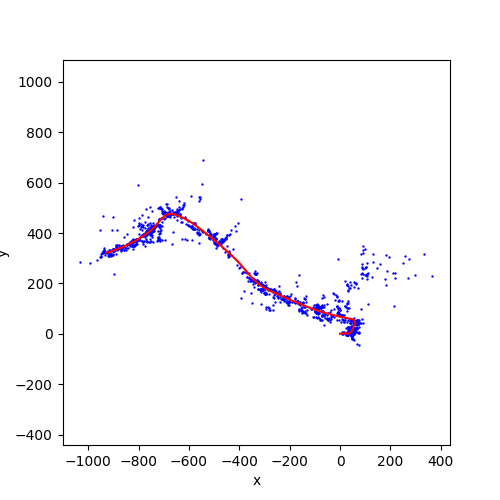
\includegraphics[width=2.5in]{../figs/03_lmk_update.png}
            % \caption{}
        \end{minipage}%
    }%

    \subfigure[Dataset 10]{
        \begin{minipage}[t]{1\linewidth}
            \centering
            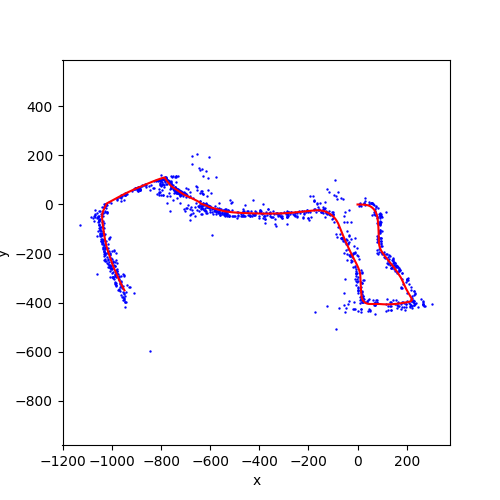
\includegraphics[width=2.5in]{../figs/10_lmk_update.png}
            % \caption{}
        \end{minipage}
    }%
    \centering
    \caption{Mapping Only} \label{fig:mapping}
\end{figure}

\begin{figure}[htbp]
    \centering
    \subfigure[03 times-index 559]{
        \begin{minipage}[t]{1\linewidth}
            \centering
            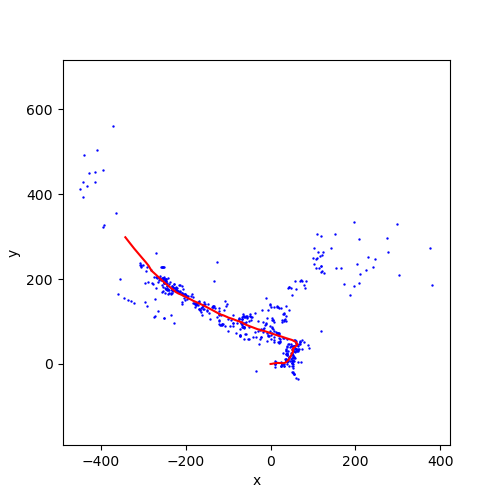
\includegraphics[width=2.5in]{../process_mapping03/03_mapping_ekf_559.png}
            % \caption{}
        \end{minipage}%
    }%

    \subfigure[03 times-index 599]{
        \begin{minipage}[t]{1\linewidth}
            \centering
            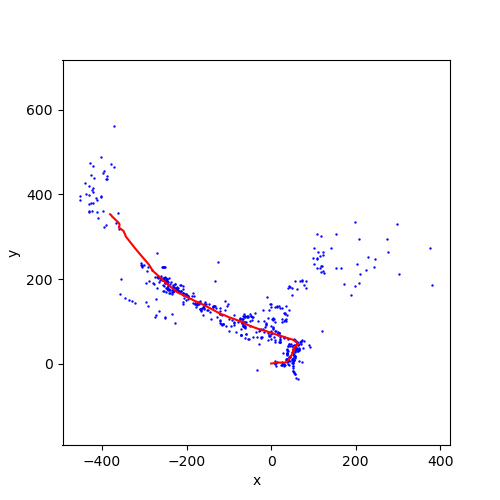
\includegraphics[width=2.5in]{../process_mapping03/03_mapping_ekf_599.png}
            % \caption{}
        \end{minipage}
    }%
    \centering
    \caption{Mapping Process} \label{fig:mapping_process}
\end{figure}

\subsubsection{Update Jointly}
The results of updating jointly are as Fig.\ref{fig:slam_joint}. For dataset 03, the trajectory does not change
so much due to shorter time and less turnings. But for dataset 10, the updated trajectory has changed significantly.
We could see how the cumulative error could make a difference to the result.

\begin{figure}[htbp]
    \centering
    \subfigure[Dataset 03]{
        \begin{minipage}[t]{1\linewidth}
            \centering
            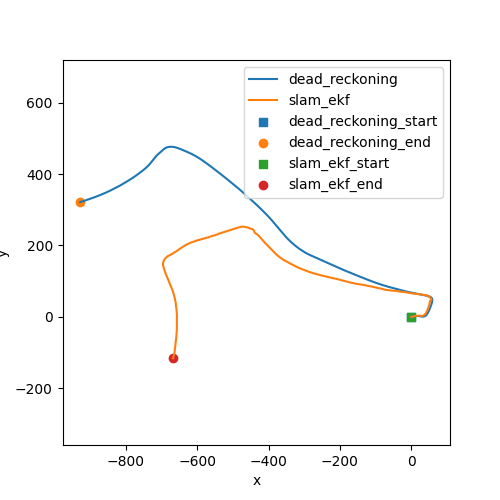
\includegraphics[width=2.5in]{../figs/03_ekf_comparison_joint.png}
            % \caption{}
        \end{minipage}%
    }%

    \subfigure[Dataset 10]{
        \begin{minipage}[t]{1\linewidth}
            \centering
            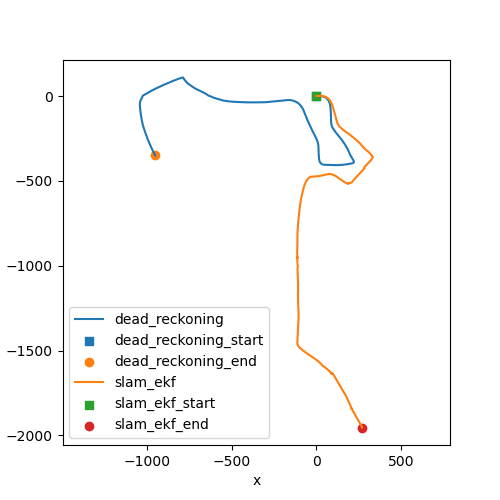
\includegraphics[width=2.5in]{../figs/10_ekf_comparison_joint.png}
            % \caption{}
        \end{minipage}
    }%
    \centering
    \caption{Update Jointly} \label{fig:slam_joint}
\end{figure}


\subsubsection{Update Separately}
If we ignore the covariance between the robot pose and the landmarks, which means that we will not use the giant overall 
mean vector and covariance matrix but two separate mean vectors and covariance matrices to represent the pose and landmarks
respectively. Thus, we would lose some information during updating step. The final results are as Fig.\ref{fig:slam_separate}.
The main difference between updating separately and jointly is the turning angle.

From the discussion above, we can see that in EKF, covariance is very important. It stores the relationship between the 
targets and observations. Ignoring such information, we could not get a good result.

\begin{figure}[htbp]
    \centering
    \subfigure[Dataset 03]{
        \begin{minipage}[t]{1\linewidth}
            \centering
            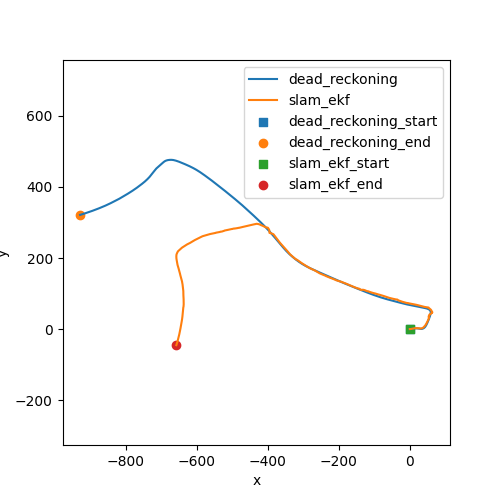
\includegraphics[width=2.5in]{../figs/03_ekf_comparison_separate.png}
            % \caption{}
        \end{minipage}%
    }%

    \subfigure[Dataset 10]{
        \begin{minipage}[t]{1\linewidth}
            \centering
            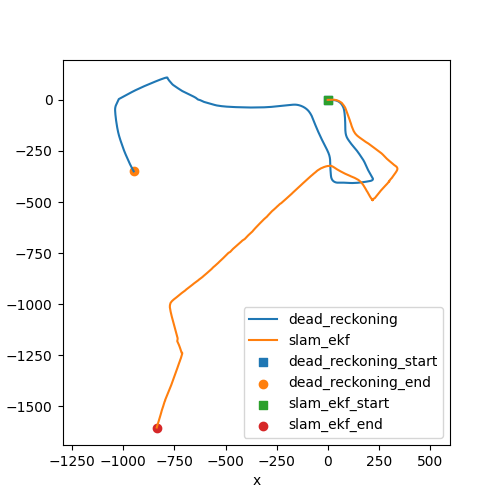
\includegraphics[width=2.5in]{../figs/10_ekf_comparison_separate.png}
            % \caption{}
        \end{minipage}
    }%
    \centering
    \caption{Update Separately} \label{fig:slam_separate}
\end{figure}

\subsubsection{Separate Landmarks}
To show that the covariance is important, we could do one more experiment, that is ignore the covariance between the 
landmarks. We view the landmarks as completely independent points, and only consider the covariance when updating the
pose. The setting leads to Fig.\ref{fig:independent}. The trajectories do not change much compared to the original ones.
Therefore, we could draw the conclusion that the covariance is a key factor when updating the pose and the map.

\begin{figure}[htbp]
    \centering
    \subfigure[Dataset 03]{
        \begin{minipage}[t]{1\linewidth}
            \centering
            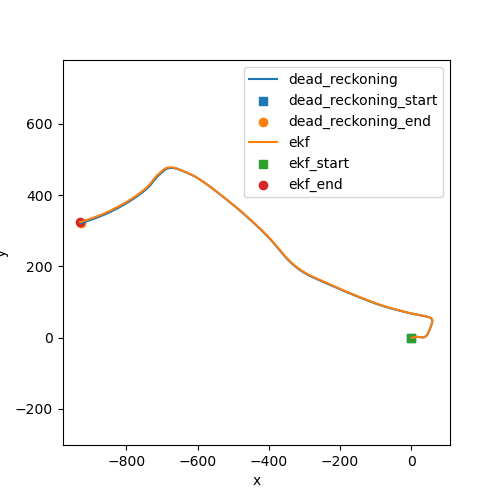
\includegraphics[width=2.5in]{../figs/03_comparison.png}
            % \caption{}
        \end{minipage}%
    }%

    \subfigure[Dataset 10]{
        \begin{minipage}[t]{1\linewidth}
            \centering
            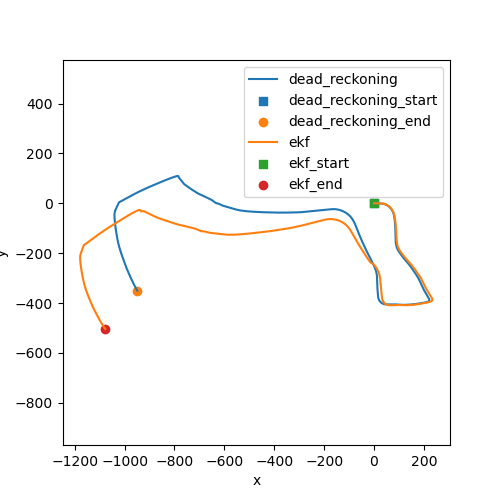
\includegraphics[width=2.5in]{../figs/10_comparison.png}
            % \caption{}
        \end{minipage}
    }%
    \centering
    \caption{Independent Landmarks} \label{fig:independent}
\end{figure}

\subsubsection{Some More Trivial Discussion}
\begin{itemize}
    \item The results also depend on the choices of the features. For example, if we choose the first 1000 features that
    are observed the most times, the trajectories would also change a little.
    \item The number of the features chosen also play a part. Choosing 800 is also different from choosing 1200. The more
    the features, the more accurate the result.
\end{itemize}

% \begin{figure}[htbp]
%     \centering
%     \subfigure[Roll for Dataset 1]{
%         \begin{minipage}[t]{1\linewidth}
%             \centering
%             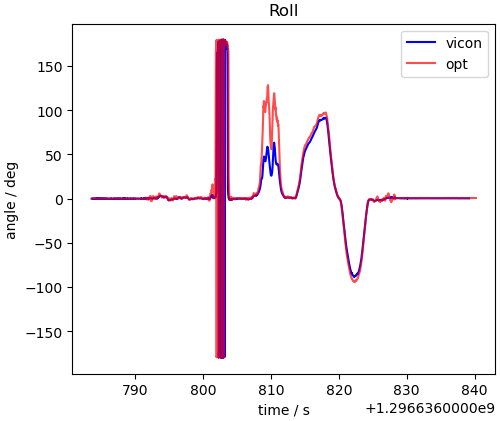
\includegraphics[width=2.5in]{../figs/Roll_1.png}
%             % \caption{}
%         \end{minipage}%
%     }%

%     \subfigure[Pitch for Dataset 1]{
%         \begin{minipage}[t]{1\linewidth}
%             \centering
%             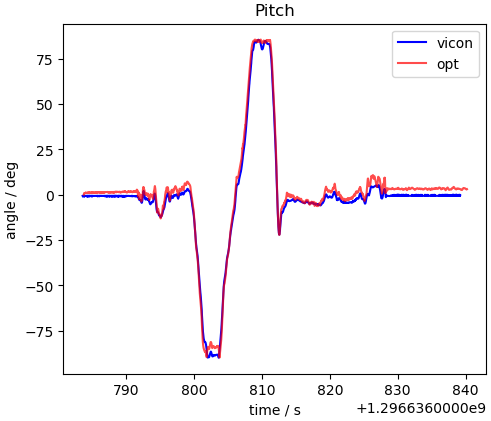
\includegraphics[width=2.5in]{../figs/Pitch_1.png}
%             % \caption{}
%         \end{minipage}
%     }%

%     \subfigure[Yaw for Dataset 1]{
%         \begin{minipage}[t]{1\linewidth}
%             \centering
%             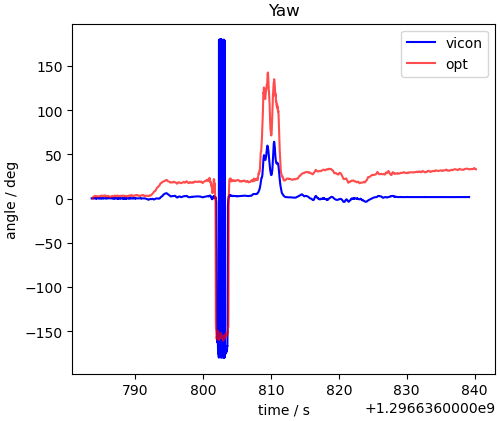
\includegraphics[width=2.5in]{../figs/Yaw_1.png}
%             % \caption{}
%         \end{minipage}
%     }%

%     \subfigure[Panorama for Dataset 1]{
%         \begin{minipage}[t]{1\linewidth}
%             \centering
%             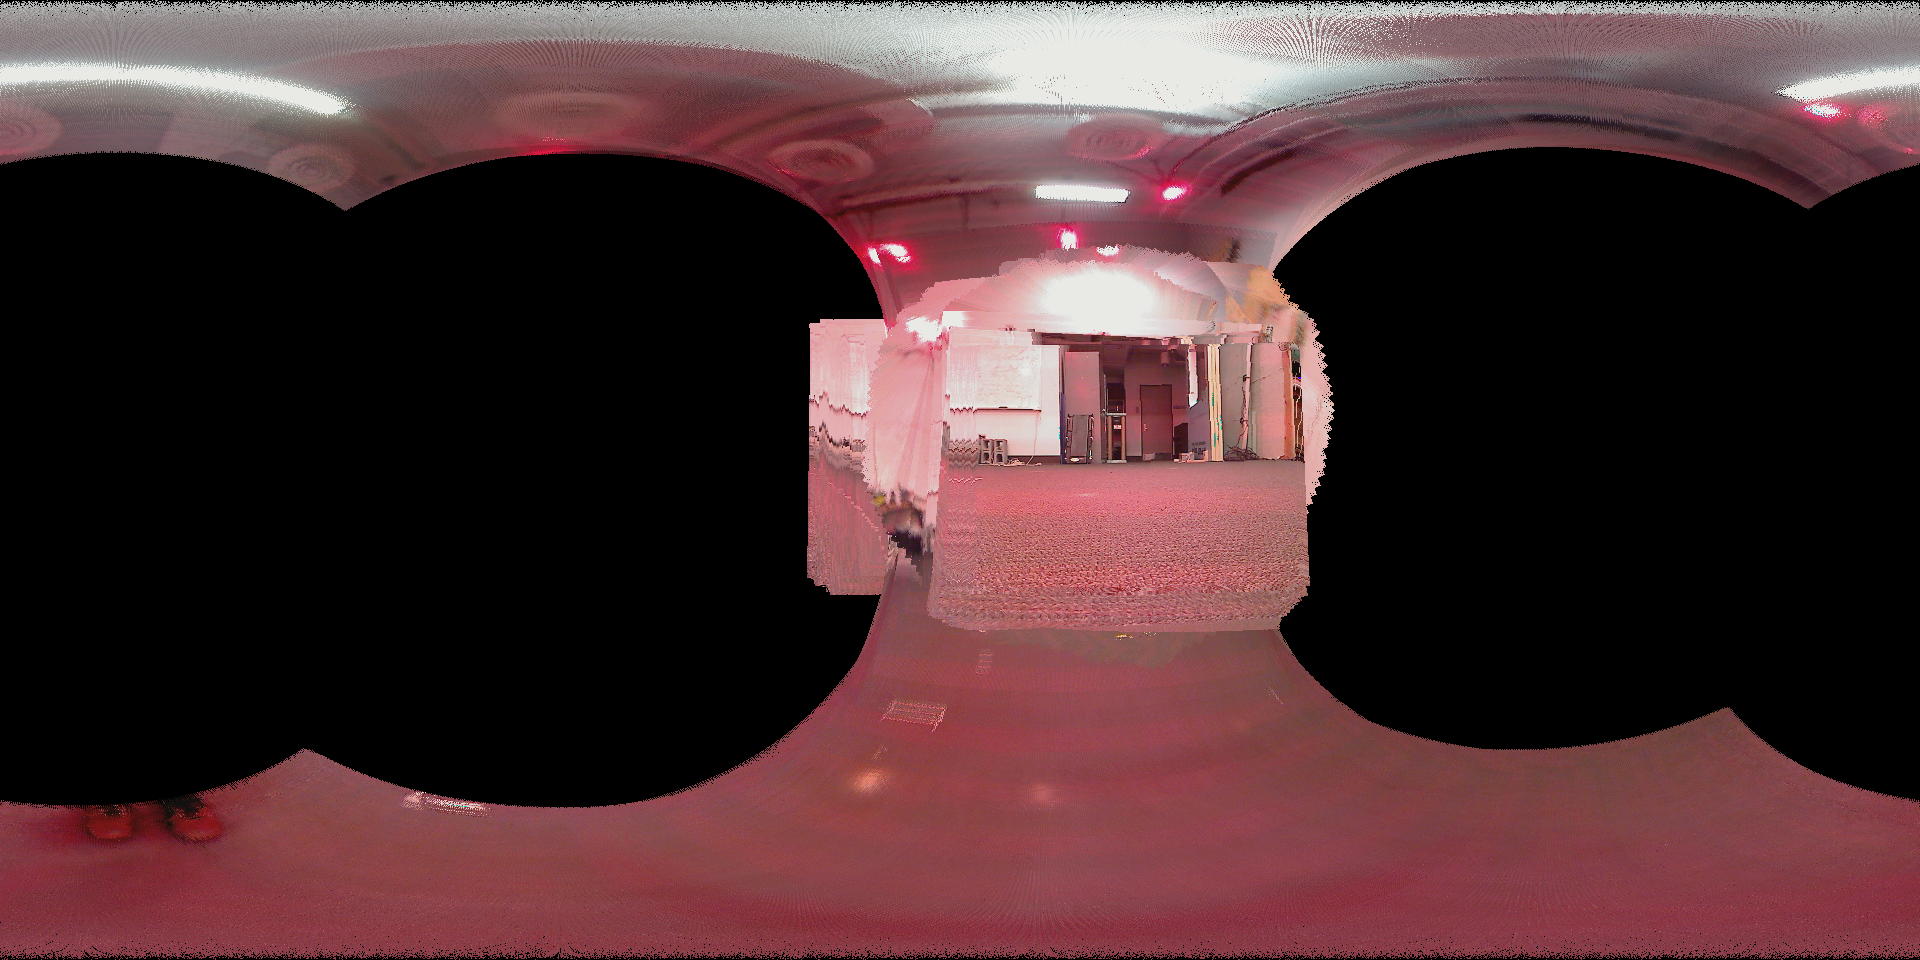
\includegraphics[width=2.5in]{../figs/panorama_1.png}
%             % \caption{}
%         \end{minipage}
%     }%
%     \centering
%     \caption{ Result for Dataset 1}
% \end{figure}

\end{document}
